\documentclass[12pt]{article}
\usepackage[margin=1in]{geometry}
\usepackage[normalem]{ulem}
\usepackage[usenames,dvipsnames,svgnames,table,xcdraw,dvipsnames]{xcolor}
\usepackage[rightcaption]{sidecap}
\usepackage{amsmath,amssymb,array,
			booktabs,
			color,
			enumitem,etoolbox,
			fdsymbol,
			hyperref,
			listings,
			makecell,multicol,multirow,
			pgfgantt,pifont,
			rotating,
			wrapfig,
			xparse
	}
\usepackage{tikz}
\usetikzlibrary{trees,tikzmark}
\usepackage{todonotes}
\graphicspath{ {./figures/} }\useunder{\uline}{\ul}{}
\newcommand{\cmark}{\ding{51}}
\newcommand{\xmark}{\ding{55}}
\NewDocumentCommand\MyInfo{O{(0,0)}O{}mmm}{
	\begin{tikzpicture}[remember picture,overlay,#2]
	\node[pin=#4:{\parbox{5cm}{\raggedright #5}}] at ([shift={#1}]pic cs:#3) {};
	\end{tikzpicture}%
}
\patchcmd{\thebibliography}{\section*{\refname}}{}{}{}
\makeatletter
\newcommand\notsotiny{\@setfontsize\notsotiny\@vipt\@viipt}
\makeatother

\begin{document}
	\begin{titlepage}
		\newcommand{\HRule}{\rule{\linewidth}{0.5mm}}
		\center
		\Large School of Electronics and Computer Science\\
		\Large Faculty of Engineering and Physical Sciences\\
		\Large University of Southampton\\[1.5cm]
		\Huge Anna Kutseva\\
		{\large 16 August, 2019}\\[3cm]
		\HRule \\[0.4cm]
		\textsc{{\huge Exploring Turing Machine Simulations on Social Machines }}\\[0.3cm]
		\HRule \\[1.5cm]
		\LARGE Project supervisor: Thanassis Tiropanis \\
		\LARGE Second examiner: Adam Prugel-Bennett \\[1.5cm]
		\Large A project report submitted for the award of BSc Computer Science \\[1.5cm]
		{\small Word count: 9956 as verified by \texttt{TeXstudio}'s `\texttt{Analyse Text}' tool}
	\end{titlepage}
	\tableofcontents
	\thispagestyle{empty}
	\newpage\vspace*{\fill}
	\begin{abstract}
	 	The more popular and widely used certain web applications and services are, the more their content, functionality, and performance revolve around their users' actions.
		The concept of social machines is becoming more and more relevant with the vast expansion of the World Wide Web, as well as the increasing user involvement in its augmentation. The basis of the former, as first suggested by Tim Berners Lee, is weaving together the creative input of various individuals with the technical processing of machines.
		However, at the time of writing there is no known way to formally define and simulate these interactions as abstract machines which fundamentally underpin our usage of the internet as a source of information composed of unknown actors. Addressing this issue, the project is going to identify the core theoretical components of social machines and build a tool for simulating the dialogue between man and machine based on formally defined behaviours.
		This will be done by implementing an architecture which utilises Turing machines and evaluating its applicability in mimicking real-life situations.
		Being able to observe socio-computational scenarios a system goes through could serve a deeper insight into the possible consequences of past, or hypothetical, design choices.
	\end{abstract}\vspace*{\fill}
	\thispagestyle{empty}
	\clearpage\vspace*{\fill}
	\begin{center}
		\section*{Acknowledgements}
			I would like to thank Jonathon Hare for the dedication to his role as my academic tutor, and the unceasing support in all forms throughout my time at university.\\[1.5cm]
			I would also like to thank M. Higgs, for his feedback, patience, positive reinforcement, and love.\\[1.5cm]
			Everyone is awesome.
	\end{center}
		\vspace*{\fill}
	\thispagestyle{empty}\clearpage
	\pagenumbering{arabic} 
	\section{Introduction}\label{sec1}
		\paragraph{Problem}\hfill\\
			Large and complex online systems no longer only involve servers performing deterministic operations; there are cases where human input is integral to completion of certain tasks or advancing through continuous processes. With the rise of the World Wide Web people have been prompted to not only interact with each other online, but with systems they can contribute to. Such systems can be classified as social machines, as the dependency of their states on the non-deterministic nature of human participants conveys the interweaving of computer logic with real-life knowledge.
			Social machines have received a fair amount of academic attention in the form of designs and frameworks to help form a more rigorous outline of their structure and behaviour. However, there are fewer attempts in developing related software for further experimental exploration and validation, and no known simulator of a formally defined social machine scheme exists at the time of writing this report.
	
		\paragraph{Goals}\hfill\\
		\label{sec:goals}
			This project aims at evaluating the feasibility of modelling social machine components via Turing machine simulations.
			There are three major stages the objective will branch into:
			\begin{enumerate}[leftmargin=*, label=\textit{Stage \arabic*}]
				\item \textbf{Analysis and specification} \\
					Based on the results of a literary review, formally define the different behaviours and components of the desired implementation, using a selection of models and classification frameworks. 
					Compose an elicitation of functional requirements regarding those findings.
				\item \textbf{Implementation} \\
					In order to ensure that all effort is concentrated on implementing original features, rather than developing a full automata simulator from scratch, elect an appropriate open source simulation framework, and extend it.
					Derive the latter's implementation prerequisites from the already established specification, but allow additions if relevant, or compromises if necessary.
				\item \textbf{Evaluation} \\
					Assess the performance, accuracy, and scientific merit of the resulting application.
					Due to the lack of example data, a set of observed and theoretical scenarios will be used to assess the algorithms, and make further conclusions about the employed model.
			\end{enumerate}
			Though principally sequential as each stage depends on the previous, it is anticipated that there may be some amount of overlap. 
			Over the course of writing this report the many iterations over its content will most likely bring additional observations.
	
		\paragraph{Scope}\hfill\\
			Clearly, this being an individual assignment bound by time strongly implies that motivations should be narrowed down to a feasibly-sized task. 
			One of the precautions taken is the aforementioned choice of building an extension, instead of a new topic-focused program.
			Another is adjusting to the insufficient amount of data by fabricating configuration cases that demonstrate the solution's ability to satisfy this project's goals specifically.
			Following review of literature it would seem that most previous endeavours into the domain have remained theoretical, which brings the need for custom data; 
			populating such an expansive dataset for testing all possible configurations would be useful, but will have to be set aside as a prompt for future work.
			Finally, the lack of practical experiments to lean on prefigures the unlikelihood of a comparative evaluation, which will also have to be left for future analysis once alternative solutions are available. 
	
		\paragraph{Structure}\hfill\\
			To begin, chapter \ref{sec2} is going to introduce the concepts leant on to formulate the basis of the problem being solved. Chapter \ref{sec3} is going to focus on investigating the knowledge acquired from the literary review and lay out the specific requirements for completing the stated goals. Thereon, chapter \ref{sec4} will document the process of fulfilling those requirements and any impediments encountered during its course. Subsequently, chapter \ref{sec5} is going to report any experimentation results with various scenarios and determine how well the final product holds up to the expectations set. Lastly, chapter \ref{sec6} will give the final run-down of the project and its outcomes, reflecting on the development process, and suggest any future work that could build on the conclusions provided.
		
		\paragraph{Ethics}\hfill\\
			Even though the topic of social machines involves, and can be used to simulate, people and behaviour, this project does not include any outside participation, therefore safety, privacy and disclosure of medical, financial, any other sort of personal or statistical data are not issues of concern.
		

	\clearpage\section{Literature Review}\label{sec2}
		\subsection{Turing Machines}	
			The initial concept of the now famous Turing machine was created as a mechanism to prove that the \textit{Entscheidungsproblem} is unsolvable~\cite{Turing1936} but turned out to have many further applications. While Alan Turing's take of machine learning~\cite{Turing1969} %original was from 1948 
			and human-like consciousness~\cite{Turing1950}, although possible in theory to emulate with state machines, were way ahead of their time, his model of abstract automatic machines contributed greatly on the foundations of the computer science field.
			
			\paragraph{Concept}
			Essentially, a Turing machine is an abstract mechanism that can be in a number of pre-defined states. These states represent literal conceptual states of a system such as awaiting input or writing to a printer of which the machine can only be in one state at a time. To keep track of past inputs and actions the machine also has a tape (of hypothetically unbound length) which represents a string of symbols (characters) with a head pointing to a specific location within that string, acting as a form of memory. To navigate between these states and manipulate information stored on the tape, the machine also has a transition function which determines which states can be moved between based on what input from the tape and what to write to the tape. This allows formal definition of all `Turing Computable' problems; i.e. all fully observable systems, like the modern computer (albeit at a very rapid rate) as defined below:
			
			\paragraph{Formal definition~\cite{Hopcroft1979}}\hfill\\\\\\\\
				\[ \Large	M= \langle Q\tikzmark{Q} , \Gamma\tikzmark{g} , \Sigma\tikzmark{s} , b\tikzmark{b}  ,q_{0}\tikzmark{q} , \delta\tikzmark{d} , F\tikzmark{f}\rangle \]
				\MyInfo{Q}{230}{\footnotesize finite set of states}
				\MyInfo[(0,9pt)]{g}{93}{\begin{center}\footnotesize complete \\ alphabet set\end{center}}
				\MyInfo[(-4pt,0pt)]{s}{270}{\begin{center}\footnotesize $\Sigma \subseteq \Gamma \setminus \{b\}$ \\ set of tape symbols\end{center}}
				\MyInfo[(0,8pt)]{b}{90}{\begin{center}\footnotesize blank symbol \\ $b\in\Gamma$ \end{center}}
				\MyInfo{q}{321}{\footnotesize  $q_{0}\in Q$ \\ start state}
				\MyInfo[(0,9pt)]{d}{40}{\footnotesize transition function \\ $\delta :(Q\setminus F)\times \Gamma \rightarrow Q\times \Gamma -  \times \{L,R\}$  }
				\MyInfo[(-5pt,3pt)]{f}{0}{\footnotesize $F\subseteq Q$ \\ set of accepting states}
				\\\\\\\\
				There are variations of this definition with regards to accepting and rejecting (halting) states, but they are widely accepted as equivalent. This one follows the definition taken from `Introduction to automata theory, languages, and computation'~\cite{Hopcroft1979}. In section \ref{sec:omega} single \textit{accept} and \textit{reject} states are used instead, following the `Introducing the $\Omega$-machine' paper~\cite{Zhang2014}.
		
		\newpage\subsection{O-machines}
			There exists a lesser known idea for an abstract machine by Turing, which was introduced in his PhD thesis - the \textit{o-machine}~\cite{Turing1938}. Similar to automatic machines, his classic and most popular abstract computational model, o-machines can be described through function tables. The main difference between o-machines and other abstract machines, such as a-machines, is the black box element, called an `oracle'. The latter's definition is not expanded upon in Turing's paper, beyond being depicted as \textit{``some unspecified means of solving number theoretic problems"}. The only specification is that no details on the internal configuration of an instance of such a machine are available, as the oracle is supposed to be capable of solving non-Turing-machine-computable\footnote{In other words - theoretically `unsolvable'} problems, such as the Halting problem, that there is no known solution for. Essentially, imagine a machine that is able to provide the solution to a given problem, but there is no way of telling how it got that solution.\\
			
			\begin{figure}[h!]
				\centering
				
\includegraphics[width=0.6\textwidth]{art}
				\caption{The computer that always has an answer?~\cite{newscientist_2014}}
			\end{figure}	

			\paragraph{Oracle Definitions}
				The typical definition of an oracle machine suggests that it is a unification of a Turing machine and an oracle, whose components are similar to those of a regular Turing machine, but also consist of unobservable internal configurations from which the function is derived. 
				
				According to van Melkebeek~\cite{Melkebeek}, an o-machine has the following components:\clearpage
				\begin{multicols}{2}
					\begin{itemize}
						\item Shared with traditional TMs:
						\begin{description}
							\item[Work Alphabet.] A set of symbols which can be written on the work tape
							\item[Work Tape.] An infinite sequence of cells that can either be empty or contain a symbol from the tape alphabet
							\item[Read/Write Head.] A component located on a single tape cell at a time that can move left or right on the work tape, as well as read and write\footnote{or delete by placing a `blank symbol'} symbols on it
							\item[Control Mechanism.] Responsible for performing actions such as moving the head, manipulating data and switching states\\\\\\
						\end{description}\columnbreak
						\item Additional components
						\begin{description}
							\item[Oracle Alphabet.] A set of symbols that may or may not be different from the work alphabet
							\item[Oracle Tape.] A semi-infinite tape of cells that can either be empty or contain a symbol from the oracle alphabet
							\item[Oracle Head.] Acts the same way as the R/W head, but on the oracle tape
							\item[\texttt{ASK} and \texttt{RESPONSE} states.] When the oracle enters \texttt{ASK} state, the current oracle tape contents are taken as a problem instance and given as an input to the oracle, which, upon finding the problem solution, replaces the work tape contents with its output; the head is moved to the beginning of the tape and the state is set to \texttt{RESPONSE}
						\end{description}
					\end{itemize}
				\end{multicols}
			
			Alternative specialist definitions of oracle machines also exist in order to abstract away the Turing Machine components. For example Adachi~\cite{adachi1990foundations} suggests an oracle that takes a tape composed only of binary symbols that can respond to ASK states with YES or NO states in a single step and as such is specialised for decision problems (e.g. ``Does the element x belong in set A?'') . In order to keep future work as flexible as possible and enable application of the oracles onto functional problems (e.g. ``What is the value of $ f(x) $?") though, this paper will focus on the extensible Turing Machine based definitions for the remainder of this project.
	

		\subsection{Social Machines}	
			The concept of a social machine is based on the idea of collaborative problem solving~\cite{Luczak-Rosch2015}. As defined by  Tim Berners-Lee, they are \textit{``processes in which the people do the creative work and the machine does the administration''}~\cite{berners2001weaving}.\\
			
			The combination of predefined machine transitions and probabilistic human input allows for introducing a plethora of outcomes for even a single system if it gets exposed to different selections of people. This is closer to the reality of modern computing, than the strict schemas of Turing machines. While non-deterministic counterparts of the latter exist, they are closer in potential to being abstract machines than actual representations of the ever-increasing and practically boundless total of branches each interaction presents in real time.\\
		
			By reinforcing connection and collaboration between people, social machines indicate existing relationships among themselves. One type of association they exhibit is belonging to one another and thus having types that can be arranged in a hierarchical tree with the World Wide Web as an infrastructure being its root (though the scope of any given tree can easily be constrained such that any given service could be the infrastructure underpinning the associated social machine) (See Figure \ref{fig:sm-tree})~\cite{Shadbolt2009}.	
			\begin{SCfigure}[1][h!]
				\centering
				\tikzstyle{every node}=[draw=black,thick,anchor=west]
				\tikzstyle{selected}=[draw=red,fill=red!30]
				\tikzstyle{optional}=[dashed,fill=gray!50]
				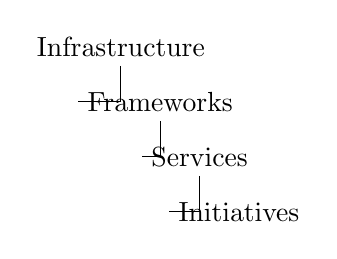
\begin{tikzpicture}[%
				grow via three points={one child at (0.5,-0.7) and
					two children at (0.5,-0.7) and (0.5,-1.4)},
				edge from parent path={(\tikzparentnode.south) |- (\tikzchildnode.west)}]
				\node {Infrastructure}
				child { node {Frameworks}
					child { node {Services}
						child { node {Initiatives}
						}
					}
				};
				\end{tikzpicture}
				\caption{Granularity levels of social machines - \textit{Initiatives} (a.k.a. \textit{Projects}) using \textit{Services} built upon \textit{Frameworks} (communication protocols) built upon the Infrastructure}
				\label{fig:sm-tree}
			\end{SCfigure}
		
		
			%\paragraph{\todo[inline]{From the semantic web to social machines: a research challenge for AI on the World Wide Web}Connects the semantic web with SMs and provides future goals~\cite{Hendler2009}}
		
			\subsubsection{Social Machine and Computation Examples}
			\label{sec:socialexamples}
			Given a lack of evaluation data found during the literature review, a few real-world social machines have been identified with the possibility of simulation by reducing the domain and action set of the oracles and machine respectively to a few representative outcomes (both positive and negative):
			\paragraph{Wikipedia}\hfill\\
			Serving as one of the most well-known cases of social machines, Wikipedia would not exist without the endless flow of human input. It confirms the capacity of social computation by being the largest encyclopaedia in existence, that is being updated at such a rate that physically publishing its content is absolutely redundant. Unfortunately, it is speculated that Wikipedia has recently been in decline~\cite{simonite2013decline}. A correct simulation of the lifetime of a similar (and preferably simplified) online collaborative knowledge project could predict tendencies in increases and declines of activity.
			\paragraph{Games with a Purpose}\hfill\\
			Undoubtedly, gamification is a powerful motivation method - simply adding a score number next to a person's username sparks the desire to increase said number. As such, it can be used to encourage meaningful contributions to a real-world broad scope problems through an entertainment platform~\cite{Ahn2006}. However, this genre of games is far from being as popular as other genres. The few notable examples that have been used to justify the importance and efficacy of GWAPs~\cite{von2008designing} are as of today defunct. Carrying out simulations of such games during their development may demonstrate potential issues, whose resolution may lead to the games' longer life and higher recognition.	
			\paragraph{The DARPA Network Challenge}\hfill\\
			The Defense Advanced Research Projects Agency organises annual prized challenges to stimulate problem solving through group effort in search of revolutionary research approaches. In 2009 DARPA presented the efficiency of social computation and crowdsourcing with the following challenge: ten weather balloons were scattered across the United States and had to be located in the shortest time possible. The participating teams used various forms of social networking to achieve their goal, and the winning team managed to complete the task in just 9 hours by putting a referral system and cash incentives to use. Many of the strategies were essentially incorporating social computation to tackle the problem in a much faster way by engaging people, rather than by setting up a massive fully automated detection system~\cite{Robertson2013}. As several of the winning strategies are publicly shared~\cite{tang2011reflecting}, they could potentially be simulated and compared given differing oracle behaviours as part of this project.
		
		\subsection{Tying It Together}
				This section has covered a number of novel automaton models and demonstrated how machines established solely on the basis of computable functions would fall flat in modelling present-day computing, considering their trademarks are \textit{interaction} and \textit{reactivity}~\cite{Goldin2004}. Having in mind the notion that interactive systems are more expressive than algorithmic ones~\cite{Wegner1997}, it is possible to look into evolving the traditional models into something more applicable to the current technological circumstances.
				 
				In the case of modelling social machines with the help of Turing's brainchildren, exploration would involve tying together the explicit automatic machines with the enigmatic potential of oracles.
				The role of a computer system in that case could then be given to a continuously executing Turing machine, with work and output tapes\footnote{Possibly an input tape as well, if determined as needed.}, allowing for indefinitely long runs of information streams.
				
				Following this, the black box characteristic of the oracles allows for assumptions about what o-machines could represent. One proposed interpretation is that a human brain can be simulated by an o-machine~\cite{Copeland1998}. Within the context of modelling social machines, a set of oracles can be utilised as stand-ins for a group of human individuals. The capacity of answering questions that a normal computer can hardly give the answer to matches with the natural unpredictability of people.
				
				Incorporating these ideas into a coherent formation has already been proposed in ``Introducing the $ \Omega $-machine''~\cite{Zhang2014}, thus presenting a straightforward prompt for exploring the matter further in the next section. 

	\clearpage\section{Problem Analysis}\label{sec3}
		In order to build any simulator, a model of the simulated environment needs to be established and followed. The first step is to break the concept in question down to its discernible parts. Then, the model chosen for this paper will be introduced, and its components will be linked to their corresponding role in the frame of the environment in question. This will help formulate the functional requirements for the practical part of the project.

	\subsection{Formalising the concept}
		So far, chapter \ref{sec2} has covered the concept of social machines, oracles and automata that can be used to model existing computer systems, but as of yet no specification has been given for how these can be joined to represent a system. Here is defined an internet-based system representing a social machine (as laid out in figure \ref{fig:sm-tree}) where the framework for communication is the passing of network data packets, the service is some modern computer system in and of itself, and the initiative is the high-level task laid out by the system's designers. This task, however, will incorporate not only the service, but a number of non-simulatable by TM actors providing some input which can easily be imagined as humans and represented by o-machines with their individual behaviours carried out by the oracles therein. If it can be theorised that the service is a Turing machine, the humans are o-machines and the data packets sent between are merely expanded symbols on a tape instead of packets on a wire then the system can be specified by an Omega Machine.
	
	\subsection{The Omega Machine}\label{sec:omega}
		The proposed implementation of a social machine model is the $\Omega$-machine, that serves as an extended model of the Turing machine, employing o-machines whose oracles act as human individuals~\cite{Zhang2014}.
		\paragraph{Dependent oracles}\hfill\\
			The initial configuration based on the omega-machine idea is:
			\[\Omega = \langle Q, \Sigma, \Gamma, \delta, q_{0}, q_{accept}, q_{reject},\Gamma_{\omega} ,\delta_{\omega}\rangle\] 
			where $\Gamma_{\omega}$ is the oracle alphabet and $\delta_{\omega}$ is the transformation function for the oracles. \\
			Upon creation, each oracle belonging to a certain omega-machine instance only needs to have its \texttt{ASK} and \texttt{RESPONSE} states be specified. In this case: 
			\[O = \langle M, s_{ASK}, s_{RESPONSE} \rangle\] 
			where $ M $ is the automatic machine that the oracle belongs to and from which it \textit{inherits} the oracle alphabet and the transformation function. 
			With this setting all oracles have identical behaviour as they have the same transformation functions (unless it's probabilistic, but then the probabilities themselves will be the same).
			The first version of the social machine model will be built following this structure.
		
		\paragraph{Divergent dependent oracles}\hfill\\
			If time allows, the the $\delta_{\omega}$ component may be broadened into $\Delta_{\omega}$, which would support a different function for each oracle instance, looking like: 
			\[O = \langle M, \delta_{\omega}, s_{ASK}, s_{RESPONSE} \rangle\] 
			where $\delta_{\omega} \in \Delta_{\omega}$, meaning there is a variety of functions that could be assigned to the oracle from a predefined whitelist, and the a-machine would be modified into:
			 \[\Omega = \langle Q, \Sigma, \Gamma, \delta, q_{0}, q_{accept}, q_{reject},\Gamma_{\omega} ,\Delta_{\omega}\rangle\]
			In this way, the oracle cluster part of the model can come closer to resembling a crowd of diverse individuals, or imagined in a smaller scale - a group whose members make different choices, but are still constrained by the system and have the same `language'.
		
		\paragraph{Independent oracles}\hfill\\
			Ideally, the ultimate configuration goal would be to have o-machines be as independent from the core a-machine as possible:
			\[M = \langle Q, \Sigma, \Gamma, \delta, q_{0}, q_{accept}, q_{reject},\rangle\]
			\[O = \langle M, \Gamma_{\omega}, \delta_{\omega}, s_{ASK}, s_{RESPONSE} \rangle\]
			where the o-machine has a reference to the a-machine, but the a-machine does not have a reference to any of the o-machines, mimicking the behaviour of a system, which is logically independent from the specific properties of its users. 
			Likewise, the behaviour of users is defined separately from the system they are tied to
			Conclusively, a social machine, or an omega-machine, can then be defined as: \[\Omega = \langle M, \mathbb{O} \rangle \] The pairing of the two serves as a communication layer between $ M $ as technical platform, or the \textit{machine} part, and $\mathbb{O}$ as the set of oracles, or the \textit{social} part. 
	
		\paragraph{Summary}\hfill\\
				Since the definition of a Turing Machine is already globally accepted, the set of oracle components are the variant sub-components of an Omega machine that determine their implementation here.
				Each definition is an extension of the prior, and each trends towards oracles having more autonomy, independent of the Turing Machine core specification.
				As shown below, Omega Machines whose oracles are either dependent or divergent are essentially an extension of the classic Turing Machine, however in the case of Omega Machines with independent oracles the Turing machine is simply an element of the overarching system.
			\begin{table}[h!]
				\centering
				\scriptsize
				\begin{tabular}{>{\centering}m{2in} >{\centering}m{2in} >{\centering\arraybackslash}m{2in}}
					Dependent & Divergent & Independent \\
					$ M = \langle Q, \Sigma, \Gamma, \delta, q_{0}, q_{accept}, q_{reject} \rangle $  &  $M = \langle Q, \Sigma, \Gamma, \delta, q_{0}, q_{accept}, q_{reject} \rangle $  & $ M = \langle Q, \Sigma, \Gamma, \delta, q_{0}, q_{accept}, q_{reject},\rangle $ \\
					$\Omega = M \parallel\Gamma_{\omega} \parallel \delta_{\omega} $ & $ \Omega = M \parallel \Gamma_{\omega} \parallel \Delta_{\omega}$ & $ \Omega =  M \parallel \mathbb{O}  $ \\
					$ O = \langle M, s_{ASK}, s_{RESPONSE} \rangle $ & $ O = \langle M, \delta_{\omega}, s_{ASK}, s_{RESPONSE} \rangle $ & $ O = \langle M, \Gamma_{\omega}, \delta_{\omega}, s_{ASK}, s_{RESPONSE} \rangle $ \\
				\end{tabular}
			\end{table}
		
	\clearpage\subsection{Specification}
		\subsubsection{Requirements Elicitation}\label{sec:req}
			Having established the formal mathematical definitions to use for modelling social machines within this project, it now falls to laying out a set of specifications that will guide the implementation of the framework.
			These goals are listed in order of importance rather than anticipated implementation order (red being an absolute must through to green being optional if time allows) as some pieces of functionality may be desirable and useful during implementation, but not critical to regard the software overall a success with relation to the goals defined in chapter \ref{sec:goals}:
			\vfill
			\begin{table}[h!]
				\centering
				%\small
				\begin{tabular}{m{3in} m{0.5in} m{2.5in}}
					Define Turing Machines & \begin{center}\textcolor{BrickRed}{$\largeblackcircle$}\end{center} & Preferably via GUI\\
					Define Omega Machines & \begin{center}\textcolor{BrickRed}{$\largeblackcircle$}\end{center} & The model itself can be simple, as long as every oracle is connected to the main Turing Machine \\
					Define the behaviour of an oracle & \begin{center}\textcolor{BrickRed}{$\largeblackcircle$}\end{center} & It should be possible to either pick from a whitelist, or ideally describe through user input \\
					Simulate the execution of a Turing machine& \begin{center}\textcolor{BrickRed}{$\largeblackcircle$}\end{center} & Base it on an input state from each oracle; show the final output; show the output to each oracle\\
					Continuously simulate the execution of an Omega machine & \begin{center}\textcolor{BrickRed}{$\largeblackcircle$}\end{center} & Demonstrate the input and output between each oracle including multiple executions; include communications between oracles\\
					Save Turing Machines & \begin{center}\textcolor{Dandelion}{$\largeblackcircle$}\end{center} & Preferably via common transferable object serialisation format \\
					Save Omega Machines & \begin{center}\textcolor{Dandelion}{$\largeblackcircle$}\end{center} & Full hierarchical specification including internal objects specifications and meta-data \\
					Save oracle Machines and/or oracles & \begin{center}\textcolor{Dandelion}{$\largeblackcircle$}\end{center} & Including all components as behaviours \\
					Enable connections between oracles & \begin{center}\textcolor{Dandelion}{$\largeblackcircle$}\end{center} & This requirement is tied to the rumour spreading scenario~\cite{Zhang2014}. It is not crucial for the minimal viable product, but greatly desired.  \\
					Enable stepped execution of the Omega machine& \begin{center}\textcolor{YellowGreen}{$\largeblackcircle$}\end{center} & Allow for debugging of individual oracle interactions, showing state at each step
				\end{tabular}
			\end{table}
		
		\clearpage\subsubsection{Existing Software}	
			As when considering the implementation of any piece of software, it never makes sense to reinvent the wheel unnecessarily.
			Given Turing Machines are also such a fundamental element of computer science, it makes sense that some form of design and simulation framework exist that can be taken advantage of here.
			As such, this section will evaluate existing Turing Machine design and simulation frameworks in order to get a head-start on the implementation goals laid out previously.
			\paragraph{Criteria}\hfill\\
				Deciding on a framework to extend is a virtually irreversible given the tight timeline of the project (See Table \ref{table:risk3} in Appendix \ref{sec:app}) and as such should be considered strongly before making a decision. The web contains a myriad of open source software options, most of which can be found on websites such as \texttt{sourceforge.net}. Notwithstanding, many, if not most, of those projects lack support, reviews, and proper documentation, which marks them as unsound options. To support the final choice, each option was evaluated against the following list of criteria (each with a tentative set of questions to consider):
				\begin{description}
					\item[Recognition] An acclaimed, or at least favourably reviewed piece of software promises a good groundwork for the experiment and increases the likelihood of it being built upon in future work. If the application is not particularly popular, or no information is given about its feedback, existing affiliation with any institutions increases trust in its quality.\\
					\underline{Questions to ask:} \textit{Where does the work come from? Is there any academic or industrial usage? Is the overall feedback, if any, thorough and positive?}
					\item[Language] Implementation in a modern and widely utilised language ensures quick uptake.\\
					\underline{Questions to ask:} \textit{What language is it written in? Is it an adequate choice for the task? Is it a familiar one? }
					\item[Maintenance] Proper and frequent support promises fewer performance issues and bugs. Also, large involvement with the project indicates large amount of effort, and consequently - good quality of the product.\\
					\underline{Questions to ask:} \textit{What are the activity levels on any associated forums or code repositories? How often have past updates been rolled out? When was the most recent update? Is the project still consistently maintained?}
					\item[Features] A large code-base reduces the need to implement basic or common features.\\
					\underline{Questions to ask:} \textit{What are the exclusive features, if any? How are machines stored? Is the program expressive enough to be extended efficiently? Are there components that can be reused in multiple ways? Is there any trivial or desirable for the project functionality missing?}
					\item[Documentation] Well commented code will be easier to work with; any additional instructive materials, such as help pages, example tutorials, readme files, or full manual documents provide evidence of usability and accessibility; thorough change logs give more insight on development, and further inform about handled or potential issues.\\
					\underline{Questions to ask:} \textit{What documentation is provided, if any? Is there a dedicated website, user manual, or a readme file? Are there any examples or tutorials? Is there a comprehensive change log for recent updates? Is the code well commented?}
					\item[Additional factors] Any extra details that do not fall into the aforementioned categories are noted separately. They are not as deal-breaking and mostly reflect aspects that may not directly affect the goal, but are worth mentioning. \\
					\underline{Questions to ask:} \textit{What is the user experience like? Are there any specific requirements to use the software? Are there any peculiarities?}
				\end{description}
			\paragraph{Options}\hfill\\
				 On the next page is a selection of ten contenders that were considered.
			\paragraph{Review and choice}\hfill\\
				 The majority of open source projects available are implemented in Java and have user interfaces built with the Swing toolkit. After inspecting the source code contents and considering factors such as support, functionality, public feedback and quality of documentation, it was strongly decided in favour of JFLAP~\cite{rodger2006jflap}, as it excelled in all the aforementioned requirements in comparison to the rest of the projects. In fact, its diverse functionality and multitude of classes for any sub-entity that might be needed will enable easier and cleaner implementation of the social machine model.
		\clearpage\begin{table}[h!]
			\centering
			\caption{}
			\label{table:open-source} 
			\scriptsize
			\begin{tabular}{|m{0.8in} |m{1in}|m{0.5in}|m{0.8in}|m{0.8in}|m{0.6in}|m{0.8in}|}
				\hline
				\textbf{Option} & \textbf{Recognition} & \textbf{Language} & \textbf{Maintenance} & \textbf{Features} & \textbf{Docs} & \textbf{Extra notes} \\ \hline
				\textit{JFLAP}~\cite{rodger2006jflap} 
					& Educational software by the Duke University.\newline The creator has been recognised as an ACM Distinguished Member \newline Widely used - most popular candidate.
					& Java 
					& Available since 1996 but still being updated;\newline the latest release is from 2018, running on Java 8  
					& Simulations for numerous other topics on automata and formal languages;\newline XML files with a custom \texttt{.jff} extension 
					& Dedicated website, books, papers, video tutorials 
					& Comprehensive class hierarchy; UI in Swing. \\ \hline
				\textit{Tursi}~\cite{schätzle_2014} 
					& Creator in\newline AIS, University of Freiburg & Java &  Written in 2013;\newpage v1.1 released in 2014 
					& Custom .tm files; Exporting tables to state diagrams, history and break states, wildcards;\newline Console mode option & Dedicated website with FAQ and a manual  & UI in Swing \\ \hline
				\textit{Owen's Turing Machine Simulator}~\cite{kellett} 
					& Used by Rensselaer RAIR Lab for testing and debugging while working on the `Busy Beaver Superpaper'~\cite{rossnew}
					& Java & Last updated in 2005 (according to file properties, no change log available)  & Save the execution of a TM over time;\newline Custom .tmo files. & Comments & It seems to be an internal project;\newline UI in Swing \\ \hline
				\textit{Tuatara}~\cite{satyr9_timestokes_2007} 
					& The only project in the SourceForge selection with several recent downloads, and a review. & Java & Last modified in 2007  & \textit{Basic} & \texttt{Help} tab within app, very short readme file, comments & Screenshots of Windows XP; UI in Swing.  \\ \hline
				\textit{TMSimulator}~\cite{archonius_hugork_2010} 
					& Made by students from the technical university of Vienna. & Java & Available since 2010;\newline Last modified in 2011 & \textit{Basic} & A readme file & The only Java UI in JavaFX instead of Swing. Lots of typing and spelling errors  \\ \hline
				\textit{Alan}~\cite{neuber_pahl_seichter_2005} 
					& A second term programming project at the University of Applied Sciences Rosenheim
					& Java &Last modified in 2005  & \textit{Basic} & SourceForge hosted website, function docs within the app, German documentation & The only project in the SourceForge selection to have a customised web page \\ \hline
				\textit{TURING MACHINE}~\cite{ugarte_2017} 
					& A list of 29 institutions are listed are allegedly using the project, according to its website  & JavaScript\newline {\tiny (jQuery)}  & Copyleft 2017  & Runtime adjustable simulation speed & Tutorial PDFs, example machines  & Web-based;\newline Clean, modern interface \\ \hline
				\textit{JSTuring}~\cite{morphett} 
					& Made by a mathematics tutor and lecturer at the University of Melbourne
					& JavaScript\newline {\tiny (jQuery)} & Initially committed in 2014;\newline Latest commit is from 2018. & Uses plain \texttt{.txt} files; saved machines are stored as Gists & Syntax explanations, some example machines & Web-based. \\ \hline
				\textit{Tm}~\cite{eck} 
					& Made by a staff member of Hobart and William Smith Colleges, Department of Mathematics and Computer Science
					& HTML5\newline {\tiny (inline\newline JS \& CSS)} & Original Java implementation dates back to 1996;\newline current version is from 2017  & Hard-coded sample machines &  A help page & Web-based. All the code is in a single \texttt{.html} file \\ \hline
				\textit{TuringSym}~\cite{jmarcost_2004} 
					& No feedback or uses found  & Delphi & Last modified in 2004 & \textit{Basic}  & Not even comments & For Win32;\newline Variable and function naming in Spanish \\ \hline
			\end{tabular}
		\end{table}

	
	\clearpage\section{Method}\label{sec4}
			With a clear set of specifications established based on the surrounding literature review, this chapter will cover the design and implementation of the extension of the JFLAP automaton design and simulation framework to include Omega machines.
			Design section \ref{sec:design} will cover a class-level overview of existing components and work to be done to achieve a functional software implementation while attempting to compensate for potential setbacks, while the Implementation section (\ref{sec:impl}) will focus on the development environment and specific implementation details noted as part of the development process.
	\subsection{Design}
	\label{sec:design}
		\paragraph{Existing tools for Turing machine creation}\hfill\\ 
			The first step towards defining Omega machines is to allow definition of the core persistent Turing machine, re-using as many of the existing JFLAP components as possible.
			JFLAP uses a directed graph-style GUI, connecting labelled states (vertices) via transition functions (edges) that are each labelled with a table of symbols to read per tape (as the branch requirement necessary to be fulfilled in order to traverse the edge), write per tape and direction of head movement per tape.
			As described before, the GUI is built in Java Swing, meaning that each change to the machine is drawn (via the \texttt{gui.viewer.AutomatonDrawer} class) onto a \texttt{javax.swing.JPanel}, all of which is contained within a \texttt{gui.environment.AutomatonEnvironment} which manages the event driven interactions that trigger when the viewing Pane needs to be redrawn, in order to accurately reflect the current state of the machine.
			States and transitions are managed in the GUI by a set of tools listed under the \texttt{gui.editor} package. The \texttt{ArrowTool}, \texttt{DeleteTool}, \texttt{TransitionCreator} and \texttt{StateTool} are of primary interest.
			Most of these are fairly self-explanatory - creating or removing components within the environment. The \texttt{ArrowTool}, however, is the general attribute manipulation tool, which inspects the component that it is being used upon, in order to provide a context-aware menu for manipulating properties.
			This can be as benign as changing labels, or associated with more core functionality such as marking initial and final states, or modifying the transition function definitions directly.
		\paragraph{Object-oriented Omega machines}\hfill\\
			As defined in section \ref{sec:omega}, the desired Omega machine model is primarily composed of a persistent Turing machine core and a number of oracle machines to interact with.
			However, to more discreetly define the relationships between oracles (for example when modelling Rumour Spreading~\cite{Zhang2014}), it would also be useful to be able to select which oracles are neighbours (using an undirected graph-style UI similar to that of the Turing Machine).
			For encapsulation, any new components created as part of this project will be kept within the \texttt{social} package, and any non-trivial additions to other classes will be described as appropriate (i.e. changes to object factories and other such boiler-plate code will not be listed).
			As such, at a high level the \texttt{OmegaMachine} class can be defined as an object which will contain a single \texttt{automate.turing.TuringMachine} representing its core, with a set of labelled \texttt{OracleMachine}-s, and a set of bi-directional connections between them.
		\paragraph{Recycling JFLAP components for Omega machine creation}\hfill\\
			Similar to the set of tools defined for manipulating Turing Machines, new tools for registering Omega Machine components will need to be added.
			Some of the existing tools will need to be extended to recognise these new components such as \texttt{DeleteTool} and \texttt{ArrowTool}, as they will need to be able to identify and display the new functionality based on the indicated component type and register subsequent changes.
			For creation, though, it will be simplest to implement dedicated tools, given these will represent entirely new components and containers.
			For example, while the PTM core of the Omega machine is really no different from a standard Turing Machine, the tool will need to be able to register either an existing Turing Machine definitions file, or create a new one, and then open a new environment for editing the Turing Machine directly (using the existing tools), while registering these changes with the parent OmegaMachine.
		\paragraph{File structure}\hfill\\
		\begin{wrapfigure}{l}{0.5\textwidth}\label{fig:lie-omega-bb}
			\begin{center}
				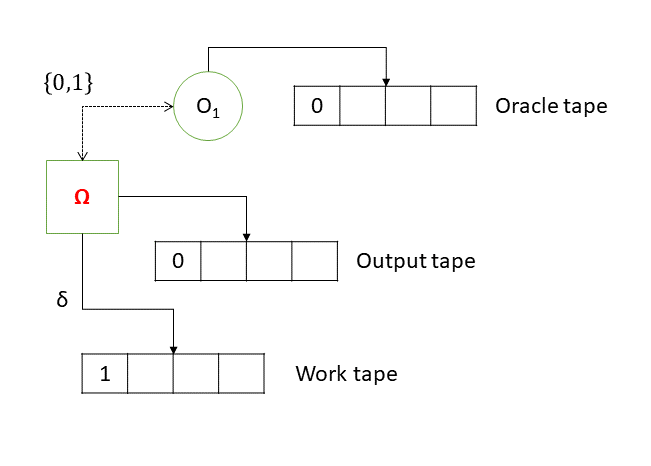
\includegraphics[width=0.5\textwidth]{lie-omega-bb}
			\end{center}
			\caption{Lie-detector structure}
		\end{wrapfigure}
			Using these components, the simplest functional Omega Machine example that could be built is a lie detector, consisting of a single oracle which the core TM will send a symbol to, asking the question ``What symbol did I just send you?''. If the oracle responds with the correct symbol then the TM outputs \texttt{0}, indicating the oracle lied, or \texttt{1} otherwise.
			In this example, the Turing Machine will consist of 3 tapes (input, output, and communication with the oracle), 4 states (\texttt{init}, \texttt{transmit}, \texttt{false}, and \texttt{true}), and 3 transitions functions (writing a symbol to the oracle and reading either a matching or non-matching symbol from the oracle). Its structure mirrors figure \ref{fig:lie-omega-bb}
			This is already representable by the \hyperref[fig:tm-xml]{XML}\footnote{Even though JFLAP saves files with \texttt{.jff} extension, they  are, regular XML files} below:\clearpage
			\lstset{
				language=xml,
				tabsize=8,
				%frame=lines,
				frame=shadowbox,
				rulesepcolor=\color{gray},
				xleftmargin=20pt,
				framexleftmargin=15pt,
				keywordstyle=\color{blue}\bf,
				commentstyle=\color{gray}\it,
				stringstyle=\color{OliveGreen},
				numbers=left,
				numberstyle=\tiny,
				numbersep=5pt,
				breaklines=true,
				showstringspaces=false,
				basicstyle=\notsotiny,
				keywords = {
					type,tapes,automaton,machine,ptmCore,state,transition,
					omSet,oracleMachine, structure, x, y, label,
					initial,final,from,to,read,write,move
				},
				emph={
					id,name
				},emphstyle={\color{red}}
			}\newpage
			\lstinputlisting[label={fig:tm-xml}]{figures/binary-TM.jff}
			In order to enable re-use of an encompassing Omega Machine in a similar manner, an \texttt{OmegaTransducer} will need to be implemented. It will parse and write XML to build to / save from an \texttt{OmegaEnvironment}.
			
			As part of this transducer, the existing \texttt{file.xml.TMTransducer} can be used to save \hyperref[fig:tm-xml]{the XML from the Turing machine} as the core, as demonstrated in \hyperref[fig:omega-xml]{the shown Omega machine XML file}:\newpage
			\lstinputlisting[label={fig:omega-xml}]{figures/binary-Omega.jff}\clearpage
		
		\paragraph{Running simulations}\hfill\\
			Once everything is loaded, simulation of the automata can be initiated. In JFLAP, a Turing Machine under active simulation is represented by \texttt{automata.turing.TMConfiguration}.
			This configuration is generated at the start of simulation, based on the provided definition and inputs, containing the current ``state'' (i.e. current TM state and tape contents) and all information required to step through the machine (i.e. all other TM states and transition functions).
			For execution, though, the \texttt{automata.turing.TMSimulator} is responsible for indicating accept states and managing execution flow, at the most basic level checking branch conditions based on current overall state and applying transition steps to the configuration.
		\paragraph{The execution loop}\hfill\\
			The Omega Machine simulations will function very similarly, though it will not be possible to directly extend the \texttt{TMSimulator} class as much of its functionality is implemented in-line, as opposed to being exposed via \texttt{protected} helper functions. To keep the project scope reasonable, existing code will not be refactored (especially given the pervasiveness of \texttt{MERLIN MERLIN MERLIN} comments in this class indicating unsavoury practices).
			However, extending the \texttt{TMConfiguration} class will be possible, as this is simply a container for TM-related member variables, which can be wrapped with the Omega machine context.
			As described above, this context will contain a number of oracle machines, each of which may have their own behaviour. To allow for this, and to take the unrestricted black-box implementation into account, the oracles should run arbitrary Java code when requested to execute by the \texttt{OmegaSimulator}.
			With this in mind, and in order to take into account the persistent nature of the core, the execution loop for the Omega machine will be as follows:
			\begin{enumerate}
				\item Simulate the Turing Machine in line with the existing JFLAP simulation loop, treating writes / reads to tapes $3..n$ as \texttt{ASK} / \texttt{RESPOND} calls to oracles $1..n-2$
				\item When the simulation reaches a `final' state within the TM, execution will be passed to each of the oracles in turn, along with the information left to them on their read / write tapes
				\item After the oracles complete their execution, the TM will re-run from its `initial' state but retaining all tape contents from prior executions, including modifications by oracles
				\item These steps will loop until the TM reaches a `final' state with no symbols on any tape except for the output tape, indicating there is no more work to be done and the machine has reached an `accept' state.\footnote{Termination is not a compulsory step - the machine can run indefinitely long, similarly to a web application with an unknown lifespan.}
			\end{enumerate}
		\paragraph{Gossiping neighbours}\hfill\\
			To include communication between oracles (such as in the rumour-spreading scenario described by Zhang et al.~\cite{Zhang2014}), a \texttt{gossip} interface can be exposed on the oracles alongside \texttt{execute}, to be called as part of neighbouring oracles' execution cycles. 
			This will require an oracle to be aware of its neighbours, but then the oracles will be free to communicate as many times as necessary during their execute cycle via a tape I/O interface, like that of the core Turing Machine.
		\paragraph{Stepping through the execution of an Omega machine}\hfill\\
			The last sub-task, as laid out in section \ref{sec:req}, is to enable debugging and tracing of Omega Machine executions.
			JFLAP again provides the base elements required via the components listed above for execution and state tracking, in tandem with the \texttt{gui.sim.SimulatorPane}, which contains a \texttt{gui.sim.ConfigurationController} for monitoring and stepping through states.
			Luckily, this \texttt{ConfigurationController} uses the more standardised \texttt{automata.Configuration} interface for manipulating state, and as such should require minimal modification to also work on \texttt{OmegaConfiguration} objects.
			Manipulating the \texttt{SimulatorPane}, however, may be more difficult as the \texttt{OmegaMachine} can be viewed from both inside the Turing machine and at the oracle interaction layer, potentially requiring greater environment manipulation or conceptualisation.
			As such, this will be left as the final implementation stage before completion, potentially being left for future work.
	\subsection{Implementation}
	\label{sec:impl}
			Having explored the components available for building a Social Machine design and simulation framework, and identified the work required to achieve the goals set out in chapter \ref{sec:goals}, implementation can now begin.
			A functional product is one of the key deliverables of this project, in order to enable acceleration of future work concerning Social machines, as such this section will list key details discovered during implementation to assist with continuing to build upon the framework laid out here.
			As the majority of the class specifications were set out in section \ref{sec:design} though, it is not necessary to re-enumerate every class and function call.
			This section will, instead, focus on required tools and libraries, and significant changes / issues encountered on implementation compared to the design phase.
		\paragraph{Setup}
			This reference implementation of our Omega Machine design framework is made available on GitHub~\cite{AnnaKutsevaGitHub}, based entirely on freely accessible tools and libraries.
			The project was built using Eclipse 2019-03~\cite{eclipse_2019}, using the Java SE-1.8 JDK~\cite{java_8} and a number of Apache SVG manipulation libraries that are required to compile and run JFLAP~\cite{maven}.\footnote{Required libraries are: \texttt{batik-dom-1.7.jar}, \texttt{batik-svg-dom-1.7.jar}, \texttt{org.apache.batik.ext.awt.1.6.0-20081006.jar}, \texttt{org.apache.batik.svggen-1.6.0-20081006.jar} and \texttt{org.apache.batik.swing-1.6.0-20070705.jar}.
			It should be noted that these versions are specifically required due to JFLAP incompatibilities with newer version APIs.}
		\paragraph{Restrictions}		
		\begin{itemize}
			\item[\xmark] \textbf{XML structure:\\}
				Transducing machines was particularly difficult, not because of XML complexity, but the structure of the existing transducer logic.
				While XML DOM (Domain Object Model) manipulation libraries are in use within JFLAP, the existing code elects primarily to work from the root node of the object as opposed to relative nodes.
				This lead to some issues with the nested TM core, as data points, such as the number of tapes available, were expected in the root machine node rather than as part of the individual automaton, requiring specific workarounds as part of the \texttt{OmegaTransducer} to address.
				In future, it is considered that the \texttt{ISerializable} interface could be used along with the more modern XML manipulation APIs, to automatically generate and read from structured data based on class specifications, rather than needing to manipulate XML elements directly.
			\item[\xmark] \textbf{Tape count limitation:\\}
				An unanticipated limitation of JFLAP is the hard-coded limit of 5 tapes on a Turing Machine. In chapter \ref{sec2}, it is suggested that each oracle is supposed to have 2 tapes (input and output) for communication with the core.
				However, if this is strictly followed, alongside an input and output tape for manipulating the core itself, the machine can only ever have a single oracle network, which obviously will not suffice.
				Upon lifting this limit though, it is immediately obvious why this restriction is in place, because having too many tapes per transition function (See fig.\ref{messy-tapes}) becomes unwieldy, potentially taking up the entire GUI with the tapes required for a single transition on larger networks, making it difficult for the user to identify which tapes map to which use-cases.
				\begin{SCfigure}[0.25][h!]\label{messy-tapes}
					\centering
					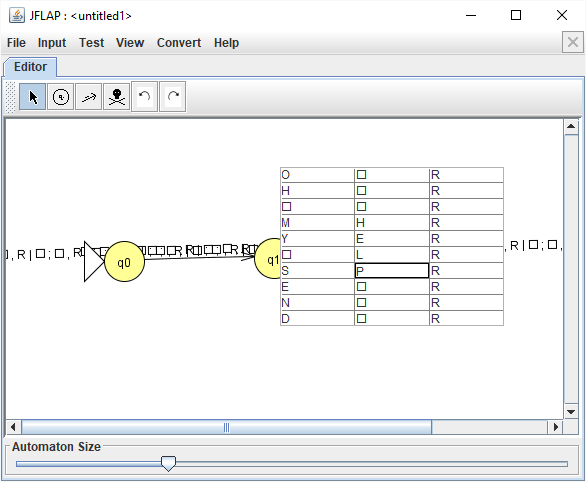
\includegraphics[width=0.55\textwidth]{messy-tapes}
					\caption{An example of a 10-tape T-machine, with only 3 states, the last of which is obscured by the transition table}
				\end{SCfigure}
				Similarly, one could look in the opposite direction: as any multi-tape Turing machine can be represented by a single-tape one, as could the interactions with oracles be read from a single tape at pre-defined offsets.
				This again, however, would become infeasible with larger networks, both on the simulation side, navigating back and forth along the tape, and from the design perspective whereby the user would need to build this navigation logic into the Turing machine specifically tailored for the number of attached oracles.
				As a compromise, it was decided to retain a sensible limit on the number tapes available for this first foray into simulation, while also modifying the model to use only a single tape for I/O to each oracle, enabling functional small network design and simulation.\newpage
			\item[\xmark] \textbf{Code quality:\\}
				On top of the issues listed so far, there are also inevitably some that arise just from working with legacy software. In this case, they spawn from it being initially created in an older version of Java\footnote{Most likely 1.0 given the known timeline~\cite{procopiuc1996visualization}} and expanded over the years with new features put on top of ageing code without too much refactoring. Modern Object-Oriented design principles, such as generic typing, are scarcely used. Despite the plentiful commenting that mostly provides the insight needed, there are still quite a few code blocks framed with ``\texttt{MERLIN MERLIN MERLIN}" comments with no further explanation, leading to difficulty extending the software with new functionality without worrying about accidentally breaking underlying logic.
				Another contributing factor to the suboptimal nature of the framework, given that it entered development two decades ago, is the use of Java Swing, which is now an outdated graphic user interface library. The resulting GUI implementation is hundreds of Java code lines that would have been much easier to maintain and modify through, e.g. FXML files instead. It is a minor inconvenience compared to the functional elements of the code, though it may hinder development time given surrounding documentation may be out of date. Additionally, it is slightly unsightly.\footnote{Yet, most of the other simulators written in Java, all of which newer than JFLAP, use the same GUI libraries anyway, so the archaic experience is inescapable.} 
				Notwithstanding, since improving code quality is not the aim of this project, and time constraints are in place, focus has been driven towards implementing the required functionality as part of the project goals.
			\item[\xmark] \textbf{Oracle behaviours not definable at runtime:\\}
				A desirable feature identified as part of the design process for the framework was the ability to have multiple oracle machine functions as part of a single Omega machine, enabling the simulation of multiple actors in a scenario with different behaviours.
				This is implementable by specifying a \texttt{social.oracle} package from which to select, but given JFLAP is implemented in Java, there is no way to dynamically load oracles at runtime from within the language.
				The ideal representation would include a text box per oracle that can either inherit pre-defined behaviour, or allow arbitrary user customisable code for run-time interpretation which it was theorised could be implemented using Java Lambda functions; this however is not the case.
				Potential solutions are to include the JDK into the framework for compilation at simulation time to execute separately within the JVM, or calling out to a functional language interpreter sub-process (such as Python or JavaScript), but as these require extensions to the code-base too great to consider here, users requiring custom oracle functionality will need to implement it within the project directly.
		\end{itemize}
			Despite the aforementioned issues, the framework was completed to a viable degree. 
			As such, constructing social machines for simulation and evaluation can be looked into.
		
	\clearpage\section{Evaluation}\label{sec5}
		At this stage, JFLAP's Omega Machine definition and simulation framework has been built and now it falls to proving that the implementation is satisfactory based on the goals laid out in chapter \ref{sec2}, and providing metrics to improve upon in future work, given the restricted development window and compromises taken laid out in chapter \ref{sec3}.
		Given at the time of writing this appears to be the first piece of work towards \textit{simulating} social machines, there are no alternatives for comparative evaluation against, nor a collection of metrics established to measure and report for empirical evaluation.
		This section will enumerate a set of simple example scenarios, reporting on qualitative metrics for future comparative analysis against this base implementation and relating back to the goals they satisfy.
		Once complete, the section will finish with some general comments on the software's overall fit for purpose and a critical reflection.
	
	\subsection{Lie Detector}
	\begin{wrapfigure}{R}{14em}
		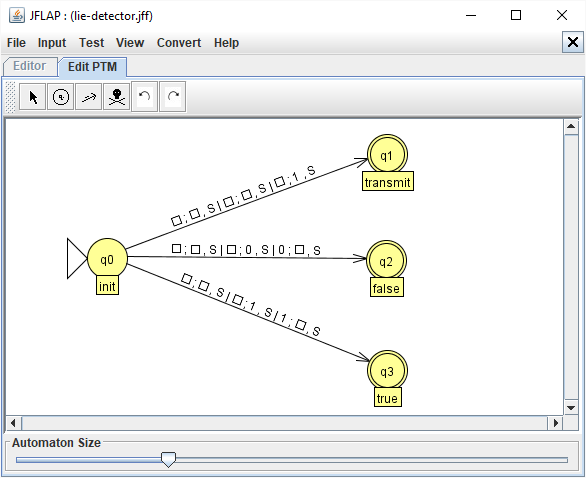
\includegraphics[width=\linewidth]{scenario-lie-tm}
		\smallskip\par
		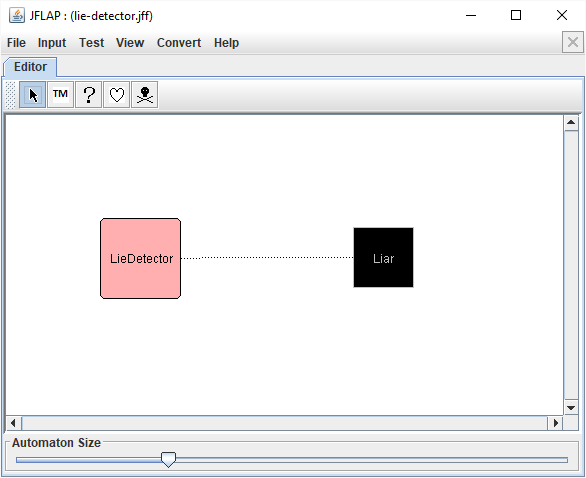
\includegraphics[width=\linewidth]{scenario-lie-omega}
		\caption{A simple lie-detecting Omega Machine}
		\label{fig:lie}
	\end{wrapfigure}
		The simplest possible $\Omega$-machine that can be defined is one with a single actor alongside the core; a useful machine concerning itself with a single unknown actor could be that of a lie detector.
		In the simplest terms, the core machine will provide the actor with a symbol and `ask' it what symbol it was passed. On receiving a response, the core will report whether this was the correct symbol (truth) or otherwise (a lie).
		To achieve this, on top of the base Turing Machine for manipulating interactions with the actor oracle, a \texttt{LyingResponderOracle} was implemented with a customisable parameter in the range \texttt{0.0-1.0} indicating the probability of `lying', and placing a different symbol back on its communication tape.
		As shown in appendix \ref{app:trace}, the software is able to not only define and simulate such a machine, but also step through the states whereby interaction with the probabilistic actor takes place while producing the expected results, satisfying goals the majority of the specification set out in section \ref{sec:req}.
		Unfortunately, this machine is so simple that there are no meaningful measurements to be derived from it, other than the responsiveness of the application (i.e. each configuration step, including those determined by the oracle, takes less than 0.1 seconds), but it still serves as a minimum requirement for any future simulator to be able to replicate this basic decision problem's definition and simulation.

	\clearpage\subsection{Collective Intelligence}
	\begin{wrapfigure}{L}{18em}
		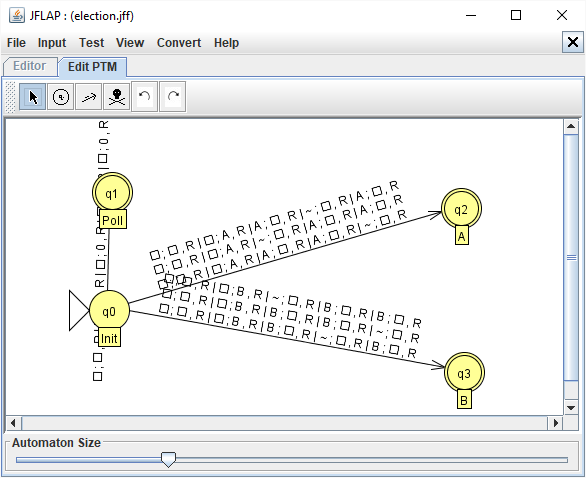
\includegraphics[width=\linewidth]{scenario-col-tm}
		\smallskip\par
		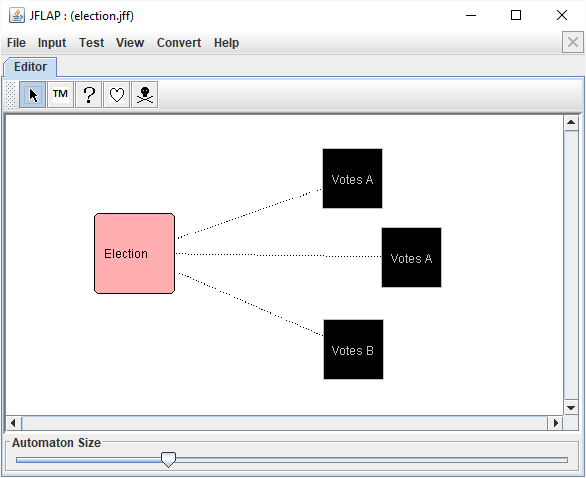
\includegraphics[width=\linewidth]{scenario-col-omega}
		\caption{A simple collective intelligence gathering Omega Machine}
		\label{fig:collect}
	\end{wrapfigure}
		In `Introducing the $\Omega$-machine'~\cite{Zhang2014}, the idea of gathering collective intelligence from a group of actors in Omega Machines is introduced, which given all of the examples depicted in section \ref{sec:socialexamples} are implementations of gathering information from unknown actors, is an important concept to cover here for comparison against future implementations.
		In this simplified example, corroboration of distributed information (as Wikipedia might be considered) could be considered a voting application whereby actors vote on the correct definition of information (in the same way individuals contribute and verify article edits).
		At a high level, the core `polls' all actors for information (though Wikipedia doesn't actively request information, this could be considered analogous to notifying interested parties to an edit of a page) on a topic, as indicated by the symbol placed on each oracle's communication tape.
		In response, the oracle replaces that symbol with a new candidate symbol representing that information in a condensed manner to be communicated back to the service. On receipt of the information, the service simply chooses the response with the most `votes' for publishing to the output tape.
		To replicate this system, an \texttt{InformationOracle} was implemented, which can be configured to hold a string of information on setup and retrieved on \texttt{ASK}ing with the corresponding symbol index to abstract away the deep knowledge acquisition process as part of researching a topic.
		On the service side, however, in order to count votes it must either be configured to track these on a work tape while iterating over oracles, or be pre-loaded with all possible combinations of votes as transition functions to the relevant output state.
		For simplicity in this example, the transition functions have been hard-coded to outputs to avoid the tape manipulation and comparison logic but neither of these implementations scale particularly well with increasing numbers of options to vote upon, nor voting actors.
		While this implementation is functional and relatively easy to understand, with $n$ possible outcomes and $m$ actors, in the worst case each poll requires evaluating $n^m$ possible transition functions or maintaining a large amount of tape manipulation logic depending on implementation.
		As such, it would be worth investigating re-usable Turing Machine sub-components and abstractions for manipulating communications with large numbers of external sources.
		
	\clearpage
	\subsection{Rumour Spreading}
	\begin{wrapfigure}{R}{18em}
		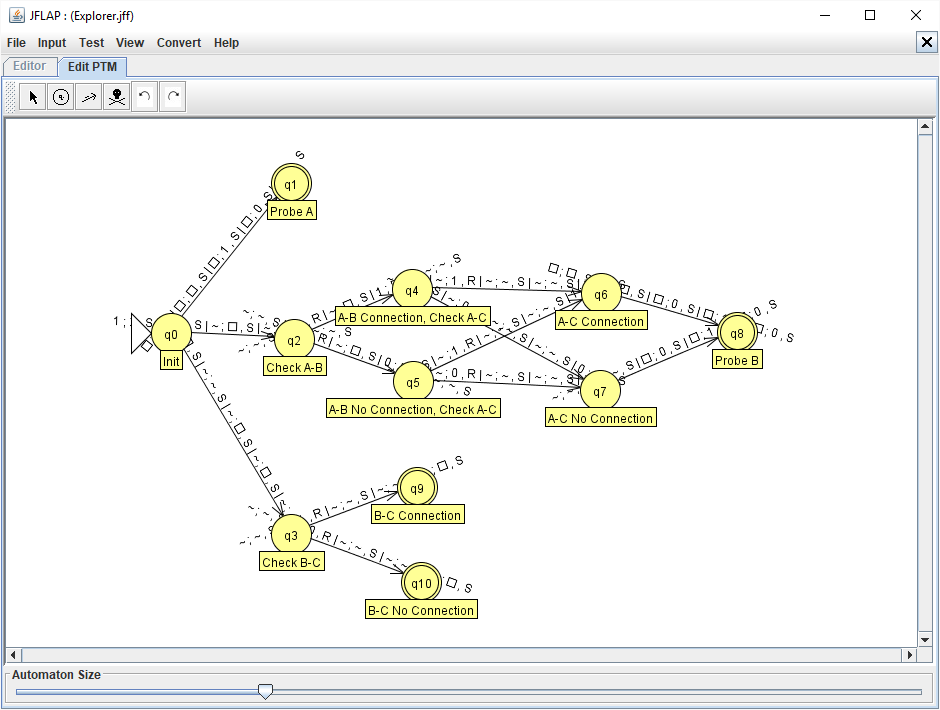
\includegraphics[width=\linewidth]{scenario-rum-tm}
		\smallskip\par
		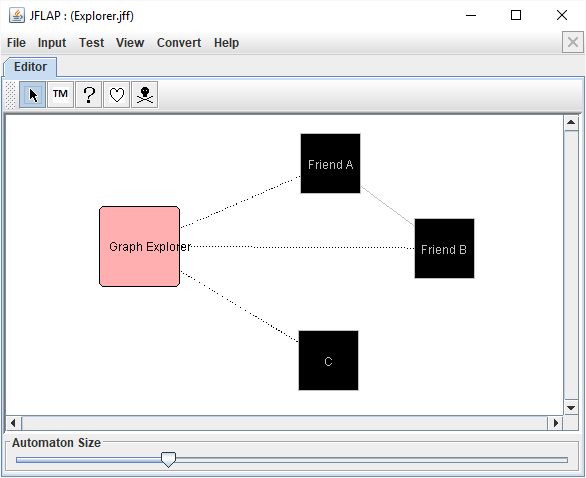
\includegraphics[width=\linewidth]{scenario-rum-omega}
		\caption{A simple rumour spreading Omega Machine}
		\label{fig:rumour}
	\end{wrapfigure}
		Another possibility of using $\Omega$-machines is to simulate rumour spreading~\cite{Zhang2014} among a network.
		This is reflected particularly well in the real world by marketing on social media platforms where each actor in a network of friends may or may not be shown an advertisement which may or may not be shared among their network and result in an observable purchase (through some tracking token).
		For this example, only a perfect product is considered\footnote{What that is however, is left as an exercise to the reader.} that is \textit{always} shared with friends and \textit{always} purchased when heard about (as implemented in the \texttt{RumourSpreadingOracle} class).
		With this information, the service can then determine connections in the network between known actors, by probing them individually as a form or graph exploration.
		To this end, the service iterates over each known actor sending them the advertisement, then after `waiting' for some time window, checking to see which actors purchased the product by placing an order on the communication tape.
		Once the orders are received, the service can then output which actors are connected by identifying which actors placed an order that were not advertised to in that iteration (see appendix \ref{app:trace} for an example trace).
		Similar to the Collective Intelligence example though, the design suffers with scale albeit more in machine complexity than time complexity.
		This derives from the fact that in the Collective Intelligence example, the machine is looking to extract the same information repeatedly from every oracle, but in this graph exploration each \texttt{ASK} and \texttt{RESPONSE} cycle needs to be context aware, meaning that for each oracle added to the network, a new set of branches for every existing execution branch on the Turing Machine needs to be added (see figure \ref{fig:rumour}).
		As such, this demonstrates the need for a component to better enable conditional looping over the set of oracles from within the Turing Machine, in order to model larger networks.\\
		It is also worth noting that the initial requirement to enable debugging of communications between oracles was not able to be implemented here.
		Given the black-box style execution of the oracles represents a single step in configuration of the overall $\Omega$-machine, it would require the implementer of the oracle to yield control back to the encompassing simulator and provide internal configuration information which is not the purpose of the o-machine as defined in~\cite{Turing1938}; meaning this is an acceptable implementation detail to be absent.
	
	\subsection{Software Suitability}
		Overall, according to the specifications laid out in section \ref{sec:req}, this project is successful as all requirements (stopping just short of debugging individual oracle interactions as part of the Omega machine) have been fulfilled by the chosen / implemented software.	
		However as part of this evaluation, a number of unanticipated deficiencies have been identified with the concept of designing Omega machines in the same way as traditional Turing machines, the most significant of which is scalability.
		In general, while social machines can be used to model interactions with a small number of unknown actors, when modelling public internet-based systems the number of actors can be anywhere from in the hundreds all the way through to millions of unique individuals.
		Each of these actors of require \texttt{almost} identical treatment, but using the current set of components available for building Turing machines, this would require a multitude of branches and large amounts of tape manipulation logic, making design at that scale infeasible.
		While one solution might be to abstract the system away again to a higher level, focussing instead on oracles representing large groups of actors and the overall result returned from a set, this is a limitation that should be acknowledged when considering the applicability of the software provided here.
		
	\clearpage\subsection{Requirements completion}
		\begin{table}[h!]
			\centering
			\small
			\begin{tabular}{m{2in} m{0.5in} m{3in}}
				Define Turing Machines & \begin{center}\textcolor{ForestGreen}{{\Large \cmark}}\end{center}& Satisfied by existing JFLAP implementation \\\\
				Define Omega Machines & \begin{center}\textcolor{ForestGreen}{{\Large \cmark}}\end{center} & Satisfied by implementation of new tools and classes on top of JFLAP definitions \\\\
				Define the behaviour of an oracle & \begin{center}\textcolor{Peach}{{\Large $ \approx $}}\end{center} & Satisfiable by creating classes within JFLAP source, but not at runtime \\\\
				Simulate the execution of a Turing machine & \begin{center}\textcolor{ForestGreen}{{\Large \cmark}}\end{center} & Satisfied by existing JFLAP implementation \\\\
				Continuously simulate the execution of an Omega machine & \begin{center}\textcolor{ForestGreen}{{\Large \cmark}}\end{center} & Satisfied by implementation of new simulation components on top of JFLAP components \\\\
				Save Turing Machines & \begin{center}\textcolor{ForestGreen}{{\Large \cmark}}\end{center} & Satisfied by existing JFLAP implementation \\\\
				Save Omega Machines & \begin{center}\textcolor{ForestGreen}{{\Large \cmark}}\end{center} & Satisfied by extending JFLAP XML transducers to include new components \\\\
				Save oracle Machines and/or oracles & \begin{center}\textcolor{Peach}{{\Large $ \approx $}}\end{center} & Class-level behaviours and parameters are saved to XML, but specific execution details are omitted \\\\
				Enable connections between oracles & \begin{center}\textcolor{ForestGreen}{{\Large \cmark}}\end{center} & Satisfied by oracle class definition and interface implementation \\\\
				Enable stepped execution of the Omega machine& \begin{center}\textcolor{Peach}{{\Large $ \approx $}}\end{center} & TM and oracle interactions observable by building on top of existing JFLAP interface, but oracle interactions and state remain unobservable to outside processes 
			\end{tabular}
		\end{table}

	\clearpage\section{Conclusion}\label{sec6}
	\paragraph{Reflection}\hfill\\
		In chapter \ref{sec1}, the interest surrounding social machines was identified, along with the utility in being able to formally specify and simulate them.
		In chapter \ref{sec2}, the building blocks underpinning automata definition were explored, leading to the choice of Omega machines as a mathematically formulated model around which to build social machines, by taking advantage of the existing software for designing and simulating similar Turing machines exhibited in chapter 
		In chapter \ref{sec4}, the class structure of the chosen JFLAP design and simulation framework was investigated and the required work to satisfy the project requirements established.\ref{sec3}.
		In chapter \ref{sec5}, predominant implementation discrepancies were identified to assist with future work upon the framework, and finally in chapter \ref{sec6} the final software was put to the test by analysing the process surrounding design and implementation of a number of example social machines with potential real world application.\\
		Following the evaluation of the completed software, a number of unforeseen factors were discovered, impacting the process of manually defining $\Omega$-machines, primarily surrounding the scalability of hand-manipulating states and transitions.
		By all accounts, the project goals and software requirements have been satisfied, but it would be foolish to announce investigation into the possibilities of modelling $\Omega$-machines complete, given the described difficulties in  implementing the example scenarios.
		It would also be short-sighted to call this project a failure, given the collation of knowledge, crystallisation of conceptual knowledge into concrete class implementations, elicitation of previously unregistered issues surrounding working with Turing machines at scale, and suggestion of potential solutions to these issues through further work.
	
	\paragraph{Improvements}\hfill\\
		Having now overseen the project to completion, if an attempt were made to re-tackle this same problem with the knowledge in-hand gained here, multiplexing features of the UI and framework itself would be the elements to focus on, as opposed to oracle simulations.
		With sufficient time, it would be a significant improvement upon JFLAP to recreate the same behaviour through an interpreted language, implementing the manipulation and simulation logic in order to promote more active development both by freeing the software from the shackles of legacy language features and libraries, and being `maintained' and distributed via an antiquated version control system, alongside better reflecting the rapidly iterative design-based goals.
		It would be unreasonable to expect a single researcher to be able to recreate this framework and achieve the results expressed in this paper within the same time span, so instead sticking with JFLAP, but creating more custom specialised state / transition amalgamation components for use within the TM cores at an early development stage, is advised.
		The only other major improvement would be to contact the social machine community~\cite{sociam} to gather and establish quantitative metrics for evaluation of the final framework, which, as well as providing a benchmark against which to compare future work, may have promoted interest in expanding upon this work by advertising it to the established community at large.

	\clearpage
	\paragraph{Future work}\hfill\\
		As previously mentioned, two major improvements on this work would be to both rewrite the existing Java code using a more modern API and putting consideration into specialised multiplexing components for manipulating functions over large numbers of oracles / tapes within Turing machines.
		However, future comparative works might centre around utilising information cascades as posited by Luczak-Rosch~\cite{Luczak-Rosch2015} to represent the same examples provided here and a similar simulation framework for modelling the transfer of information through them.
		This might (i) help identify new social machine interactions which need to be considered in order to create a fully representative model, (ii) function as an entirely independent model that makes social machines easier to design and simulate than the framework provided, or (iii) be used as part of a network representing the interactions between social machines themselves.
		
	\paragraph{Closing thoughts}\hfill\\
		All in all, this has been a successful dive into the world of system modelling frameworks and social machines, highlighting future benefits of continued research into this field, while also identifying a set of key weaknesses using the existing components that need to be rectified before the full potential of the work can be realised.
		The broad scope and potential for novel application design of social machines is an exciting opportunity to bring new knowledge to the fundamental understanding of machine modelling for computer scientists everywhere.
	
	\bibliographystyle{ieeetr}%needed?
	%\footnotesize
	\newpage
	\section{Bibliography}\label{secBib}
	
	\bibliography{bib}%\thispagestyle{empty}
	
	\newpage
	\appendix
	\section{Appendices}\label{secApp}
	\subsection{Risk Analysis}
	\label{sec:app}
	
	\begin{table}[h!]
		\centering
		\caption{Management Issues}
		\label{table:risk1}
		\footnotesize
		\begin{tabular}{|>{\centering}m{1.5in} |>{\centering}m{0.1in} |>{\centering}m{0.1in} |>{\centering}m{0.3in} |>{\centering}m{1.8in} |>{\centering\arraybackslash}m{1.8in}|}
			\hline
			\textbf{Problem}                                                 & \textbf{L}                & \textbf{S}                  & \textbf{Risk}                      & \textbf{Mitigation}                                                                                                                                               & \textbf{Contingency}                                                                                                                                                                 \\ \hline
			Falling behind schedule due to clashes with other assessed tasks & \cellcolor[HTML]{FFC702}\textit{3} & \cellcolor[HTML]{FFC702}\textit{3} & \cellcolor[HTML]{FFC702}\textbf{9} & Extra time allocated for the period surrounding exams. One hour of work allocated per day as a minimum in parallel with other modules.                            & Identify problem modules and assessments as early as possible to raise with supervisor ASAP.                                                                                         \\ \hline
			Falling behind schedule due to slow progress                     & \cellcolor[HTML]{F8FF00}\textit{2} & \cellcolor[HTML]{FFC702}\textit{3} & \cellcolor[HTML]{FFC702}\textbf{6} & Tasks defined requiring more time than estimated by default to act as an on-going buffer. Burn-down chart to be kept up-to-date for sub-goals across entire year. & Actual work should ideally run ahead of the Gantt chart given the extra time included. If falling behind then remaining work and Gantt chart should be re-evaluated with supervisor. \\ \hline
			Unavailability of supervisor                                     & \cellcolor[HTML]{ABCB00}\textit{1} & \cellcolor[HTML]{FFC702}\textit{3} & \cellcolor[HTML]{F8FF00}\textbf{3} & Maintain attendance of weekly supervisor meetings. Prepare multiple tasks to carry out ahead of time in case a meeting has to be skipped.                         & Continue with tasks as planned, maintain contact with supervisor by any means available. Contact university for support in extreme case of extended absence.                         \\ \hline
			Licensing issues                                                 & \cellcolor[HTML]{ABCB00}\textit{1} & \cellcolor[HTML]{F8FF00}\textit{2} & \cellcolor[HTML]{F8FF00}\textbf{2} & Utilise open-source software, ideally that which has already been attributed by other academic use-cases. Contact authors for permission.                         & Comply with author's requests. Publish products of project as permissible under appropriate license with referencing as necessary.                                                   \\ \hline
			Illness                                                          & \cellcolor[HTML]{F8FF00}\textit{2} & \cellcolor[HTML]{F8FF00}\textit{2} & \cellcolor[HTML]{F8FF00}\textbf{4} & Extra time buffer can be used for sick days as necessary.                                                                                                         & Re-evaluate remaining tasks as appropriate.Contact supervisor and university to advise in extreme cases.                                                                             \\ \hline
		\end{tabular}
	\end{table}
	
	\begin{table}[h!]
		\centering
		\caption{Technical Issues}
		\label{table:risk2}
		\footnotesize
		\begin{tabular}{|>{\centering}m{1.5in} |>{\centering}m{0.1in} |>{\centering}m{0.1in} |>{\centering}m{0.3in} |>{\centering}m{1.8in} |>{\centering\arraybackslash}m{1.8in}|}
			\hline
			\textbf{Problem}              & \textbf{L}                         & \textbf{S}                         & \textbf{R}                         & \textbf{Mitigation}                                                                                          & \textbf{Contingency}                                         \\ \hline
			Hardware not powerful enough  & \cellcolor[HTML]{F8FF00}\textit{2} & \cellcolor[HTML]{F8FF00}\textit{2} & \cellcolor[HTML]{F8FF00}\textbf{4} & Design model components with performance in mind. Utilising university hardware as necessary.                & Contact supervisor to request access to specialist hardware. \\ \hline
			Damaged hardware              & \cellcolor[HTML]{ABCB00}\textit{1} & \cellcolor[HTML]{ABCB00}\textit{1} & \cellcolor[HTML]{ABCB00}\textbf{1} & Ensure program and development environment are accessible from multiple sources (not just personal machine). & Utilise university hardware.                                 \\ \hline
			Loss of work (code or report) & \cellcolor[HTML]{ABCB00}\textit{1} & \cellcolor[HTML]{FFC702}\textit{3} & \cellcolor[HTML]{F8FF00}\textbf{3} & Frequent back-ups to local drives and commits to remote repositories.                                        & Retrieve latest copy from backup.                            \\ \hline
		\end{tabular}
	\end{table}
	
	\begin{table}[h!]
		\centering
		\caption{Implementation Issues}
		\label{table:risk3}
		\footnotesize
		\begin{tabular}{|>{\centering}m{1.5in} |>{\centering}m{0.1in} |>{\centering}m{0.1in} |>{\centering}m{0.3in} |>{\centering}m{1.8in} |>{\centering\arraybackslash}m{1.8in}|}
			\hline
			\textbf{Problem}                                               & \textbf{L}                                                & \textbf{S}                                                & \textbf{R}                          & \textbf{Mitigation}                                                                                                  & \textbf{Contingency}                                                                                          \\ \hline
			Chosen framework is not appropriate for implementing the model & \cellcolor[HTML]{F8FF00}\textit{2}                        & \cellcolor[HTML]{F88602}{\color[HTML]{333333} \textit{4}} & \cellcolor[HTML]{FFC702}\textbf{8}  & Appropriate analysis made before framework selection.                                                                & Implement closest approxiamation using next most appropriate tooling. Document findings regardless.           \\ \hline
			Difficulty grasping important concepts                         & \cellcolor[HTML]{F8FF00}\textit{2}                        & \cellcolor[HTML]{F8FF00}\textit{2}                        & \cellcolor[HTML]{F8FF00}\textbf{4}  & Extensive literature review before beginning implementation. Regular contact with supervisor and academic community. & Schedule additional meetings with supervisor focussed on specific topics as soon as possible to avoid delays. \\ \hline
			Insufficient methods of evaluation                             & \cellcolor[HTML]{F88602}{\color[HTML]{333333} \textit{4}} & \cellcolor[HTML]{FFC702}\textit{3}                        & \cellcolor[HTML]{F88602}\textbf{12} & Contact academic community and review any evaluation performed in available literature.                              & Discuss potential metrics with supervisor and evaluate to best of ability.                                    \\ \hline
			High algorithmic complexity                                    & \cellcolor[HTML]{F8FF00}\textit{2}                        & \cellcolor[HTML]{FFC702}\textit{3}                        & \cellcolor[HTML]{FFC702}\textbf{6}  & Review and optimise code as implemented to minimise overhead on top of underlying algorithmic complexity.            & Request access to specialist hardware to accommodate load.                                                    \\ \hline
			Poorly designed model                                          & \cellcolor[HTML]{F8FF00}\textit{2}                        & \cellcolor[HTML]{FFC702}\textit{3}                        & \cellcolor[HTML]{FFC702}\textbf{6}  & Review code with supervisor during implementation, test as soon as is feasible.                                      & Begin testing and evaluation phases as soon as possible to avoid issues with write-up due to missing data.    \\ \hline
			Bugs                                                           & \cellcolor[HTML]{F88602}{\color[HTML]{333333} \textit{4}} & \cellcolor[HTML]{F8FF00}\textit{2}                        & \cellcolor[HTML]{FFC702}\textbf{8}  & Utilise functionality tests to ensure correctness as soon as possible.                                               & Prioritise evaluation of correct work. Address issues as timing permits.                                      \\ \hline	
		\end{tabular}
	\end{table}
	
	\subsection{Contingency Plans}
	
	The table in Appendix \ref{sec:app} shows an enumeration of possible risks at an early stage during the project's life cycle and steps taken to avoid issues caused by their occurrence as best as possible. Unfortunately, having now completed the project it should be noted that a couple of these contingency plans had to be put into action due to medical issues, particularly:
	
	\begin{itemize}
		\item \textbf{Falling behind schedule due to clashes with other assessed tasks} - as the aforementioned medical issues had impact across the board on all assessments, it was necessary to contact the module assessors, as well as the project supervisor, in order to ensure visibility and plan accordingly
		\item \textbf{Illness} - extra time buffer was used as planned, then it was necessary to contact the university to arrange for extenuating circumstances
	\end{itemize}
	
	\subsection{Gantt Chart}
	See next page.
	\begin{sidewaysfigure}[]
		\centering
		\caption[Gantt chart]{Project Gantt chart.}
		\begin{ganttchart}[
			hgrid,
			vgrid={*{6}{draw=none},dotted},
			x unit=0.85mm,
			time slot format=isodate,
			vrule/.style={thick, red},
			milestone right shift = 1,
			milestone left shift = -1,
			newline shortcut=true,
			today=2018-12-11,
			progress=today
			]{2018-10-01}{2019-05-20}
			
			\gantttitlecalendar{year, month=name} \\
			
			\ganttmilestone{Initial meeting}{2018-10-08} \\
			
			\ganttgroup[group label node/.append style={align=right}]{Definition}{2018-10-08}{2018-12-23} \\
			\ganttbar[bar label node/.append style={align=right}]{Project\ganttalignnewline outline}{2018-10-08}{2018-10-11} \\
			\ganttbar[bar label node/.append style={align=right}]{Literature\ganttalignnewline research}{2018-10-15}{2018-12-08} \\
			\ganttbar[bar label node/.append style={align=right}]{Designing\ganttalignnewline the model}{2018-12-01}{2018-12-23} \\
			
			\ganttgroup[group label node/.append style={align=right}]{Implementation}{2018-11-12}{2019-02-28} \\
			\ganttbar[bar label node/.append style={align=right}]{Choosing\ganttalignnewline software}{2018-11-12}{2018-12-01} \\
			\ganttbar[bar label node/.append style={align=right}]{Familiarising with\ganttalignnewline chosen software}{2018-12-03}{2018-12-13} \\
			\ganttbar[bar label node/.append style={align=right}]{Implementation\ganttalignnewline of the model}{2018-12-14}{2019-02-28} \\	
			
			\ganttgroup[group label node/.append style={align=right}]{Evaluation}{2019-02-15}{2019-04-23} \\
			\ganttbar[bar label node/.append style={align=right}]{Functionality\ganttalignnewline testing}{2019-02-15}{2019-03-18} \\
			\ganttbar[bar label node/.append style={align=right}]{Optimisation}{2019-03-01}{2019-04-04} \\	
			\ganttbar[bar label node/.append style={align=right}]{Final\ganttalignnewline evaluation}{2019-03-18}{2019-04-23} \\	
			
			\ganttmilestone{Completed}{2019-04-24} \\
			
			\ganttbar[bar label node/.append style={align=right}]{Preparation\ganttalignnewline for the viva}{2019-04-25}{2019-05-15} \\
			
			\ganttmilestone{Presented}{2019-05-17} 
			
			\ganttvrule[vrule label node/.append style={align=center}]{\ganttalignnewline Brief deadline}{2018-10-12}
			\ganttvrule[vrule label node/.append style={align=center}]{\ganttalignnewline\ganttalignnewline Interim deadline}{2018-12-11}
			\ganttvrule[vrule label node/.append style={align=center}]{\ganttalignnewline Final\ganttalignnewline deadline}{2019-04-30}
			\ganttvrule[vrule label node/.append style={align=center}]{\ganttalignnewline Viva}{2019-05-16}
			\ganttvrule[vrule/.append style={blue, thin}]{}{2019-01-27}
			
			\ganttvrule[vrule/.append style={green, dotted}]{}{2018-12-24}
			\ganttvrule[vrule/.append style={green, dotted}]{}{2018-12-25}
			\ganttvrule[vrule/.append style={green, dotted}]{}{2018-12-26}
			\ganttvrule[vrule/.append style={green, dotted}]{}{2018-12-27}
			\ganttvrule[vrule/.append style={green, dotted}]{}{2018-12-28}
			\ganttvrule[vrule/.append style={green, dotted}]{}{2018-12-29}
			\ganttvrule[vrule/.append style={green, dotted}]{}{2018-12-30}
			\ganttvrule[vrule/.append style={green, dotted}]{}{2018-12-30}
			\ganttvrule[vrule/.append style={green, dotted}]{}{2019-01-01}
			\ganttvrule[vrule/.append style={green, dotted}]{Holidays}{2019-01-02}
			
			\ganttvrule[vrule/.append style={orange, dotted}]{}{2019-01-19}
			\ganttvrule[vrule/.append style={orange, dotted}]{}{2019-01-20}
			\ganttvrule[vrule/.append style={orange, dotted}]{}{2019-01-21}
			\ganttvrule[vrule/.append style={orange, dotted}]{}{2019-01-22}
			\ganttvrule[vrule/.append style={orange, dotted}]{Exams}{2019-01-23}
			
			\ganttvrule[vrule/.append style={green, dotted}]{}{2019-04-01}
			\ganttvrule[vrule/.append style={green, dotted}]{}{2019-04-02}
			\ganttvrule[vrule/.append style={green, dotted}]{}{2019-04-03}
			\ganttvrule[vrule/.append style={green, dotted}]{}{2019-04-04}
			\ganttvrule[vrule/.append style={green, dotted}]{}{2019-04-05}
			\ganttvrule[vrule/.append style={green, dotted}]{}{2019-04-06}
			\ganttvrule[vrule/.append style={green, dotted}]{Holidays}{2019-04-07}
			
			\ganttlink{elem2}{elem3}
			\ganttlink{elem3}{elem4}
			\ganttlink{elem6}{elem7}
			\ganttlink{elem7}{elem8}
		\end{ganttchart}
		
		\label{fig:gantt}
	\end{sidewaysfigure}

	
	\subsection{JFLAP Omega Machine Traces}
	\label{app:trace}
	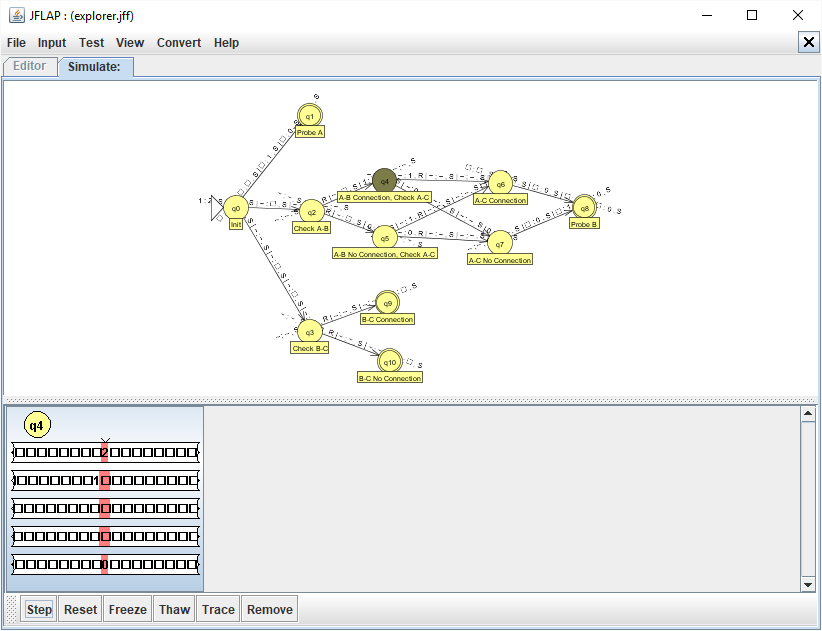
\includegraphics[width=\linewidth]{rum-tm-trace}
	\smallskip\par
	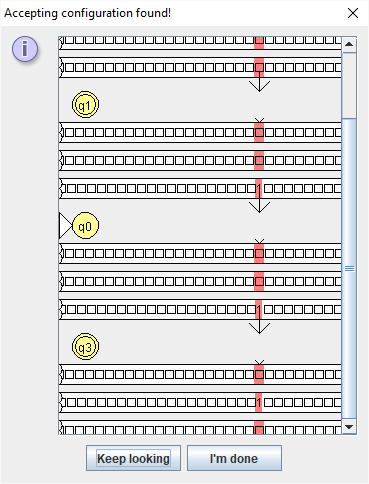
\includegraphics[width=0.4\linewidth]{lie-tm-trace}
	
	\subsection{Original Project Brief}
	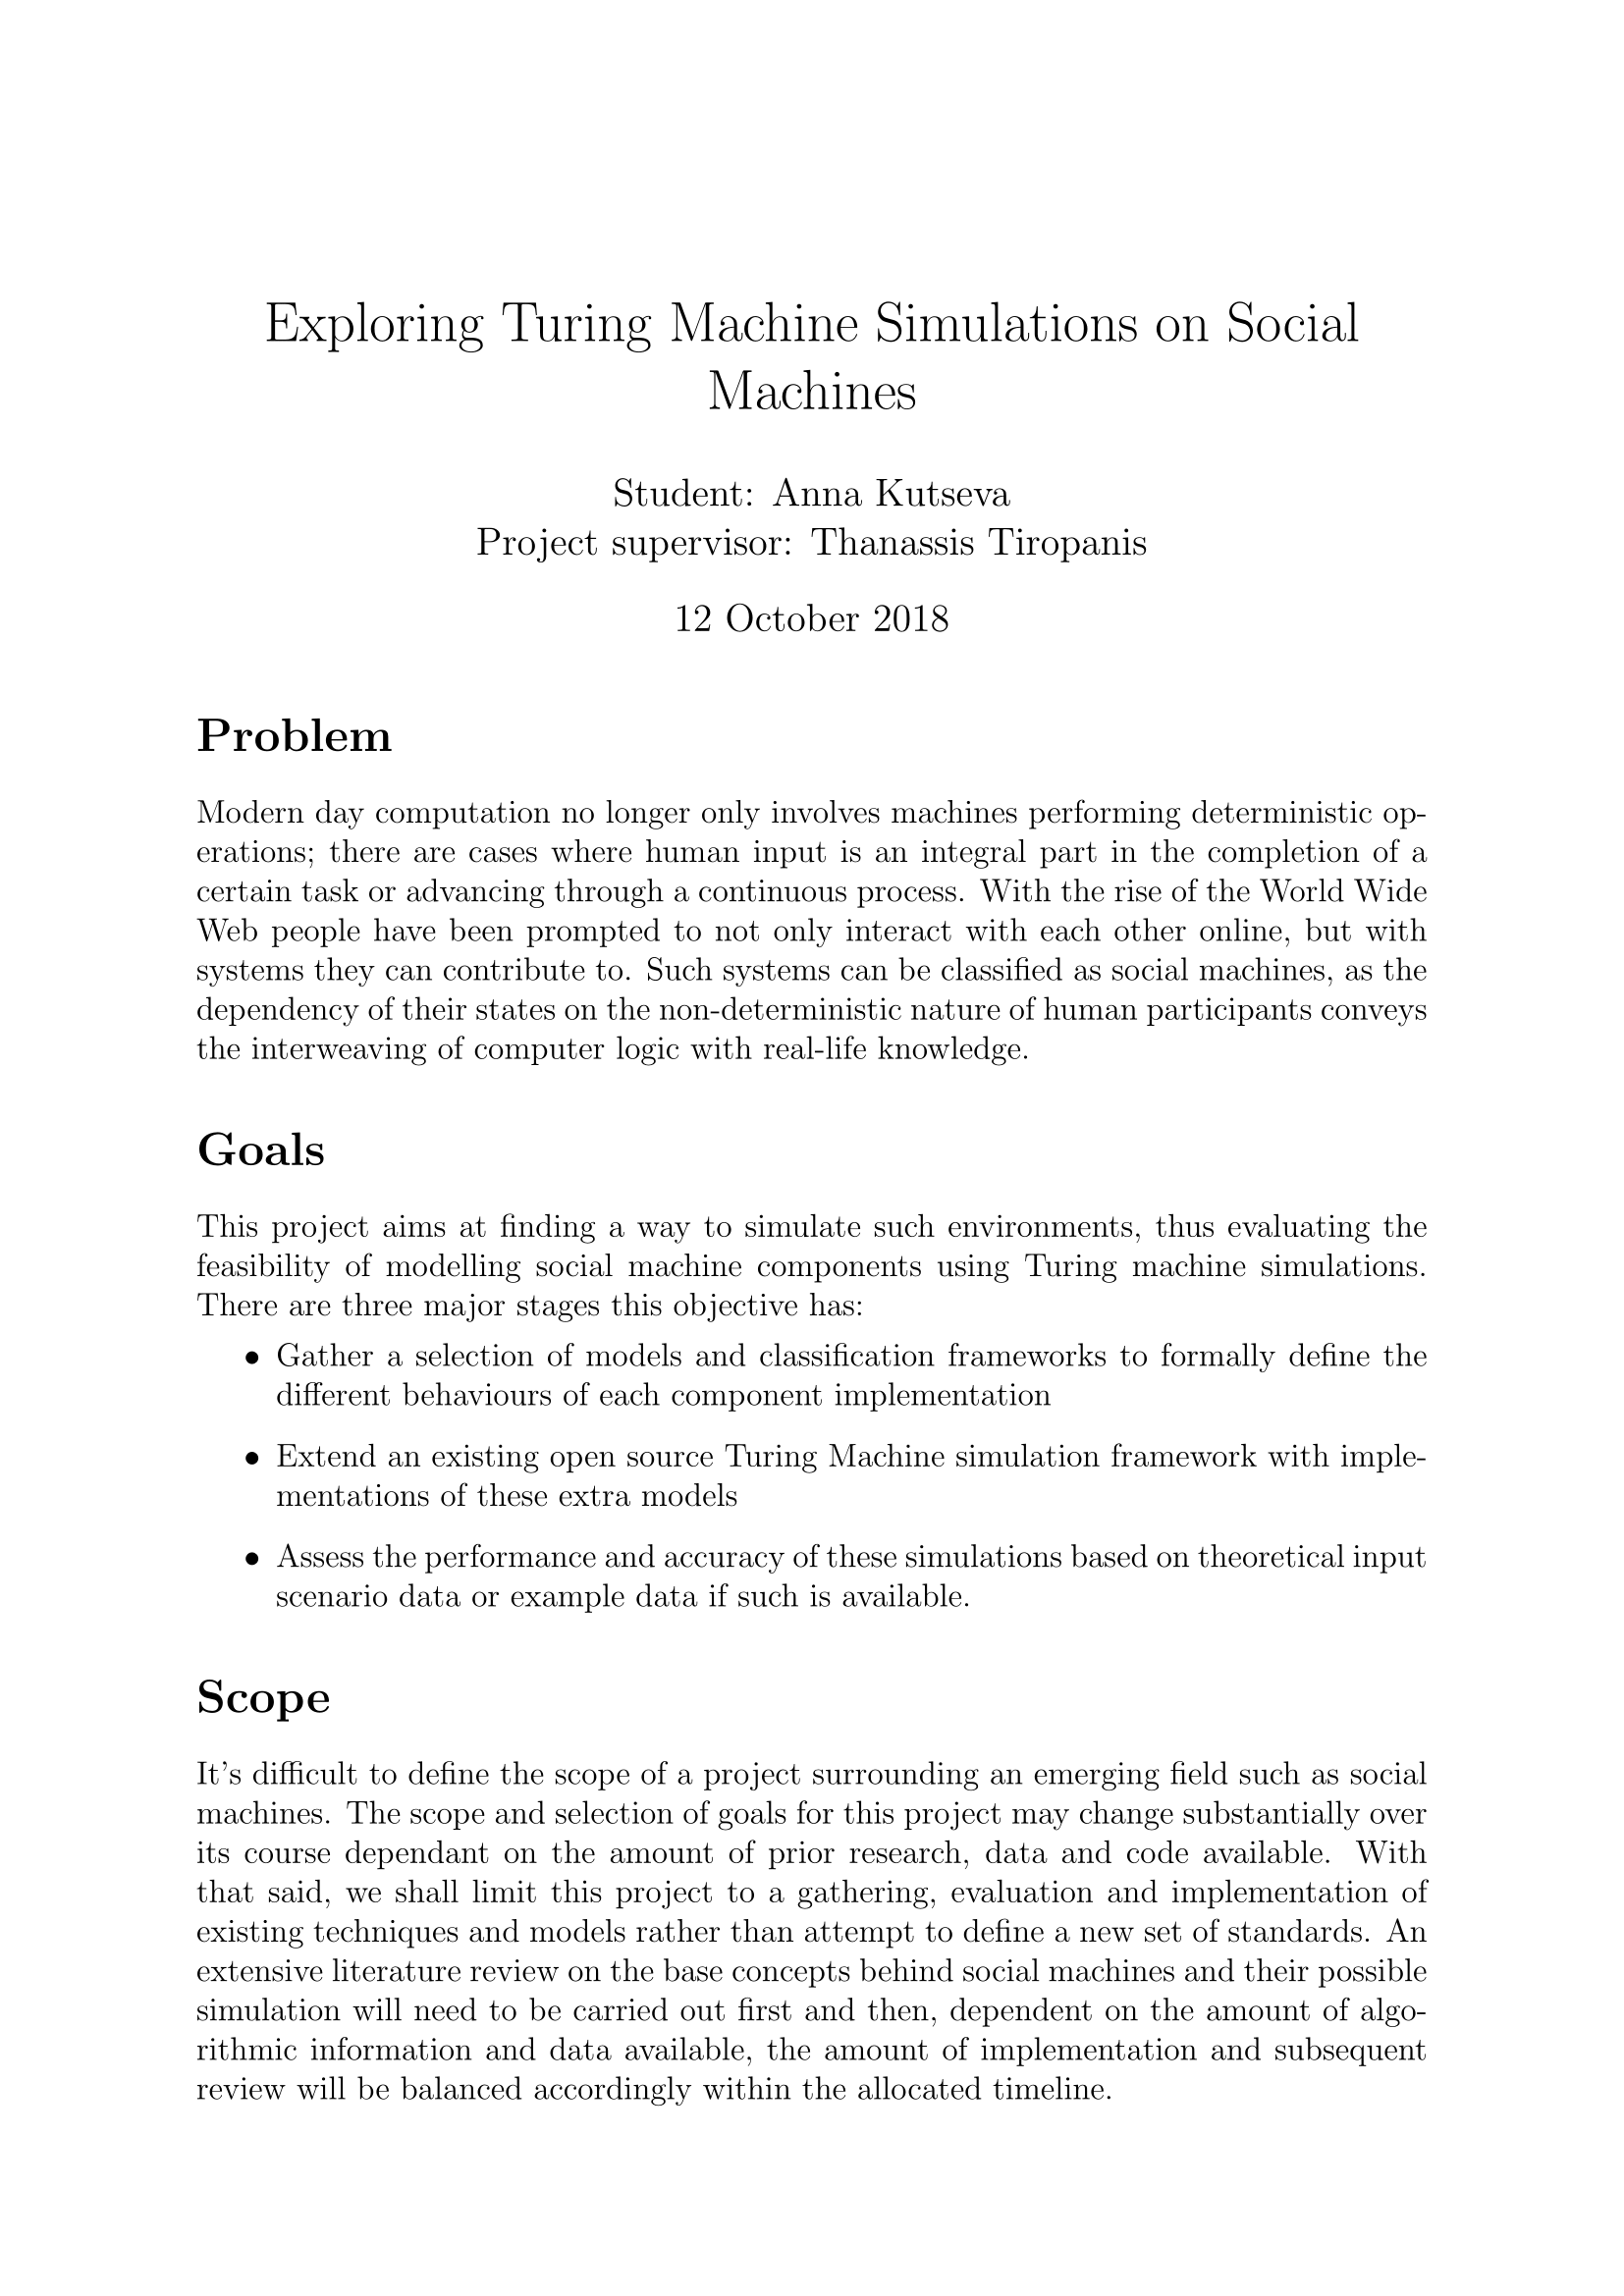
\includegraphics[width=\linewidth]{brief}

\end{document}
